\subsection{Equal-Budget Comparison of Spatial Bases}\label{sec:budget-results}
Table~\ref{tab:budget} reports the primary five-mode comparison, with 240 image-dependent scalars in place of 1,536 token entries. Ordinary token PCA retains 89.47\% of local validation advantage and 89.01\% on the historical test. Fixed spatial moments retain 81.71\% and 82.17\% under the same fixed mass and template. The corresponding increments are 7.76 and 6.85 percentage points, computed before rounding. Token PCA also exceeds DCT and all 16 random bases on both roles. The random ranges are 76.70--78.84\% and 76.38--79.38\%, respectively. The spatial-moments row uses a fixed training mass, while the template plus five residual moments in Table~\ref{tab:aggregation} uses image-specific coverage masses. This accounts for the small differences between the two tables.

\begin{table*}[t]
\caption{Retained position-control advantage (\%) at five modes including the constant. All methods use a shared fixed mass, position template, and 240 image-dependent input coefficients. View 0 is shown.}\label{tab:budget}
\centering\small
\begin{tabular}{lrrrr}\toprule
 & \multicolumn{2}{c}{Local} & \multicolumn{2}{c}{Masked}\\
Basis & Validation & Hist. test & Validation & Hist. test\\\midrule
\budgetrows
\bottomrule\end{tabular}
\end{table*}

\begin{figure*}[t]
\centering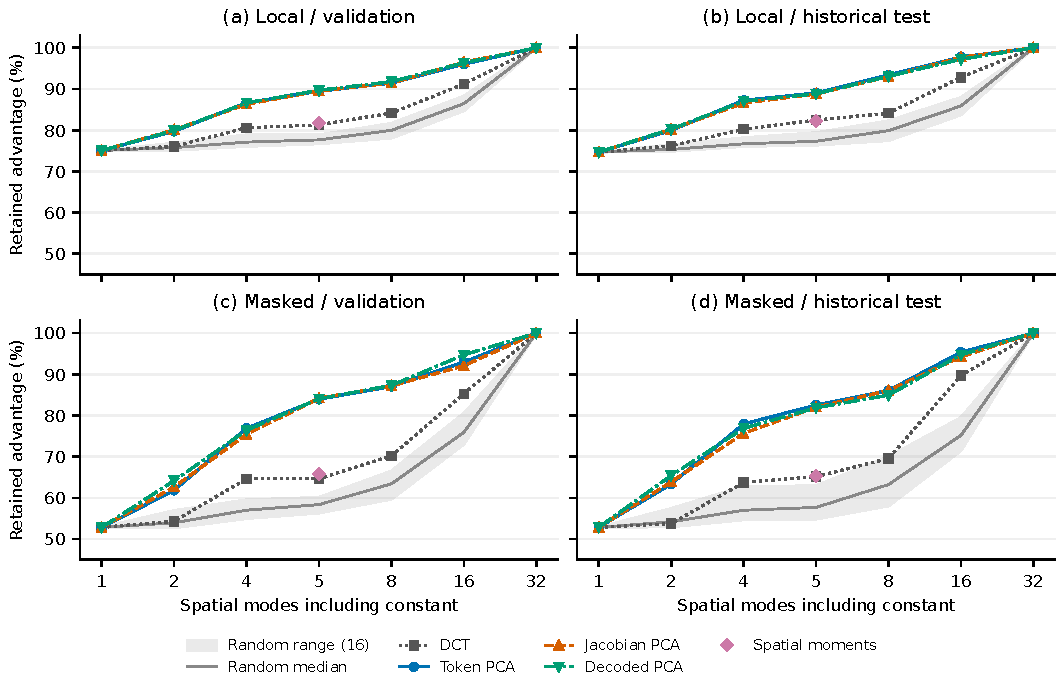
\includegraphics[width=\textwidth]{spatial_budget.pdf}
\caption{Retained advantage across the fixed spatial budget. The shaded interval is the range of 16 fixed random bases and does not represent statistical uncertainty. All methods share the one-mode and full-budget endpoints. Intermediate gaps reflect differences in the spatial basis at the same input coefficient count.}\label{fig:budget}
\end{figure*}

\begin{figure*}[t]
\centering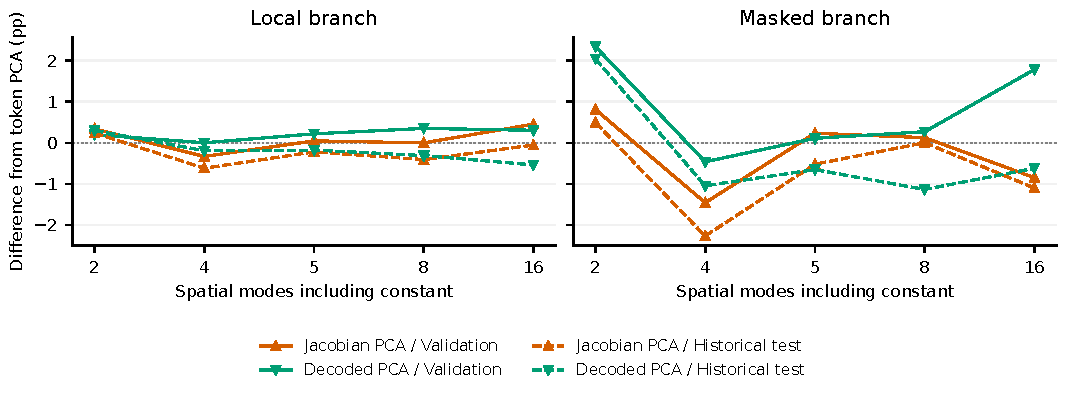
\includegraphics[width=\textwidth]{spatial_budget_differences.pdf}
\caption{Retention differences relative to token PCA at each intermediate coefficient budget. The dashed line marks equal performance. Differences are computed before rounding.}\label{fig:budget-differences}
\end{figure*}

Decoder-aware bases provide no consistent aggregate improvement over ordinary PCA. Decoded PCA improves local validation retention by 0.22 percentage points, then trails token PCA by 0.18 points on the historical test. Jacobian PCA improves masked validation by 0.23 points and trails by 0.52 points on the historical test. At five modes under view 1, the local result is nearly unchanged. Masked historical retention drops for all three fitted bases and their ordering remains token, Jacobian, then decoded PCA. The recorded views vary both appearance and mask layout. Figure~\ref{fig:budget-differences} shows the small differences concealed by the overlapping curves. At 16 modes masked validation retention is 94.72\% for decoded PCA and 92.93\% for token PCA.

The gain from fitted spatial modes also depends on the descriptor and component. At five modes token PCA reduces local validation orientation-axis loss from 0.45467 under fixed moments to 0.40166, and contrast loss from 0.62604 to 0.59896. For the historical low-proxy component it retains 80.21\% of local advantage versus 74.82\% for moments. For the historical high component the respective values are 95.42\% and 87.51\%. The remaining low/high gap shows that learned spatial modes recover some lost texture in both groups while preserving a substantial difference in retention.

\subsection{Sensitivity to Training Components and Decoder Order}
Fitting the token PCA template and basis with equal training-component weight changes five-mode local retention from 89.47\% to 89.68\% on validation and from 89.01\% to 87.92\% on the historical test. Across the six component omissions, retention spans 88.46--89.47\% and 86.45--89.01\%, respectively. All of these local values remain above the corresponding fixed-moment values. The largest historical-test reduction occurs when omitting the unresolved mid parent component, which holds the most training images. This perturbation changes both the training composition and its size, so it cannot isolate a class effect. The masked historical-test range is wider at 78.43--82.48\%. The group sensitivity is materially larger than the differences among the three five-mode PCA surrogates.

For local validation with five token PCA modes, the task-loss increase of 0.02545 separates into 0.02639 for output-space compression and $-0.00094$ for the change in order. The mean absolute difference between token-first and output-first predictions is 0.03132 on the same support. For the masked branch, this difference rises to 0.10045 while the signed order effect is $-0.00326$. Thus the nonlinear decoder changes the fields even when the signed task penalty is small. Signed loss alone would hide the extent of the prediction change. Both drift bounds hold at image level to numerical tolerance and the full-budget endpoint reproduces uncompressed predictions to within $1.5\times10^{-14}$. The independent loss reductions and source pins are described in Section~\ref{sec:repro}.
